\documentclass[a4paper,12pt]{article}

\usepackage{babel}
\usepackage[utf8]{inputenc}
\usepackage{graphicx}
\usepackage{float}
\usepackage{enumitem} 
\usepackage{hyperref}
\usepackage{caption}
\usepackage{url}
\setlength{\parindent}{4em}
\setlength{\parskip}{1em}

\begin{document}

\title{Improvise SegNet architecture with Canny edge detector algorithm for more boundary accurate image segmentation.}

\author{
  Arik Md. Isthiaque\\
  \texttt{1103096}\\
  \texttt{Section B}\\
  \texttt{Level 4, Term 2}\\
  \texttt{Department of Computer Science and Engineering}\\
  \texttt{BAIUST}
}

\maketitle

\section{Topic Characteristics}
SegNet, is an encoder decoder architecture built with deep convolutional neural network for pixel-wise semantic segmentation for images and videos. It is generally built for roads, buildings, cars, pedestrians and for differentiated the context between roads and side-walks \hyperlink{1}{[1]}. SegNet extracts low resolution pixel information from input image and classify them as per pixel. This extraction must generate some patterns which can be used in boundary localization.

Our main contribution on this paper is to study and analysis the details of SegNet encoder decoder architecture and reduce the parameters of convolutional networks and perform Canny edge detector algorithm for more boundary localized feature maps, so that it can be more memory efficient and produce more robust sematic segmentation.  

Image segmentation is a process where the objects of an image is classified by their pixel information. In an image certain pixel share some common characteristics. By identifying them we can label the pixels, so they can be detected from the image. We use image segmentation to find objects in images like text (OCR), cars (automated vehicle), cancer, tumor (medical image). In recent days, deep learning algorithms got a success in handwritten OCR, NLP  \hyperlink{3}{[3]},  \hyperlink{4}{[4]}. It has also a huge active interest for pixel-wise semantic segmentation. Recently there are some approaches are being carried out to adopt deep learning algorithm for pixel-wise semantic segmentation  \hyperlink{5}{[5]}. The results of these approaches are very encouraging  \hyperlink{6}{[6]}. But we still need better architecture to run the segmentation process. So, improvise the current architectures is needed for more robust segmentation.

\section{Working Hypothesis}
The architecture will take RGB image as input and the input will be directly fed into the encoder network. The encoder network is topologically identical to the 13 convolutional layers in the VGG16 network  \hyperlink{1}{[1]}. The network will perform convolution with a filter bank to extract a set of feature maps. Then they will go for a batch normalization process  \hyperlink{9}{[9]}. Then an element-wise ReLU will be applied. After each convolutional operation a max-pooling will be performed. Max-pooling is used to achieve translation invariance over small spatial shifts in the input image.
The most important phase of this architecture is the decoder network. Here, there is no learning involved in this network. First upsampling will be performed in the feature maps. Here the upsampling process will be performed by inverse convolution using a fixed or trainable multi-channel upsampling kernel. The final decoder output feature maps will be fed to a soft-max classifier for pixel-wise classification. After that we will run Canny edge detector for more localized boundary detection.

\clearpage

\section{Methodology}

\begin{figure}[h!]
\centering
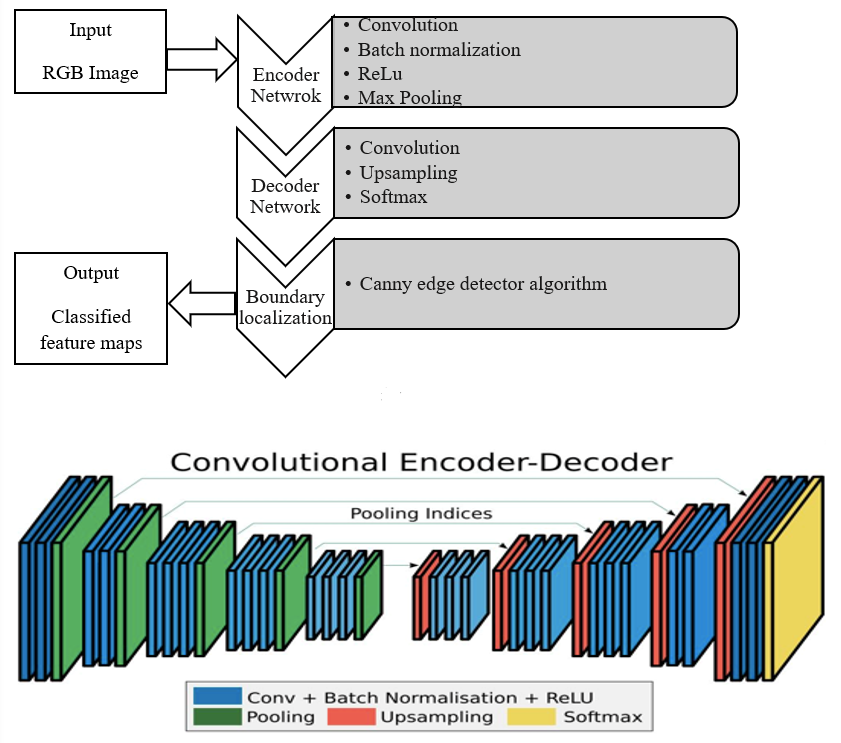
\includegraphics[width=1.2\textwidth]{fig_1.png}
\caption{The proposed methodology}
\end{figure}
\newpage
\section{Outline}

\begin{figure}[h!]
\centering
\hyperlink{1}{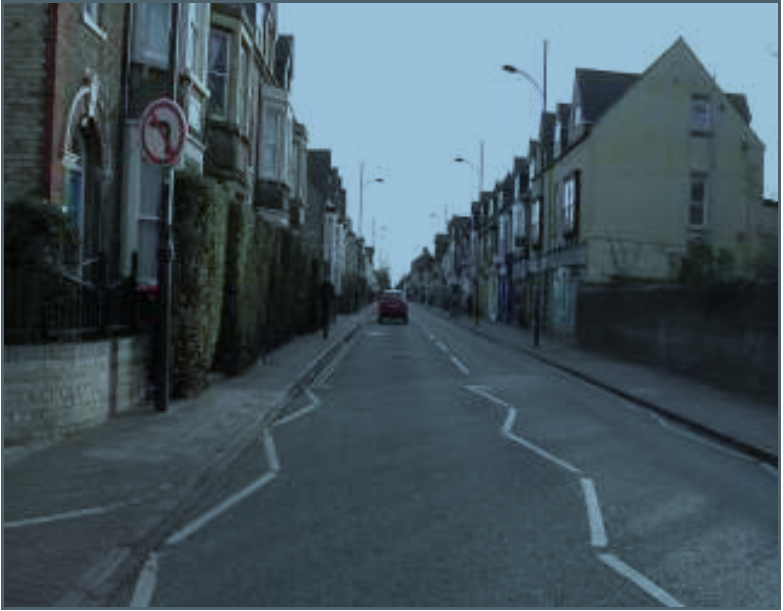
\includegraphics[width=.4\textwidth]{fig_2.png}}
\caption{Input RGB image[1].}
\end{figure}

\begin{figure}[h!]
\centering
\hyperlink{1}{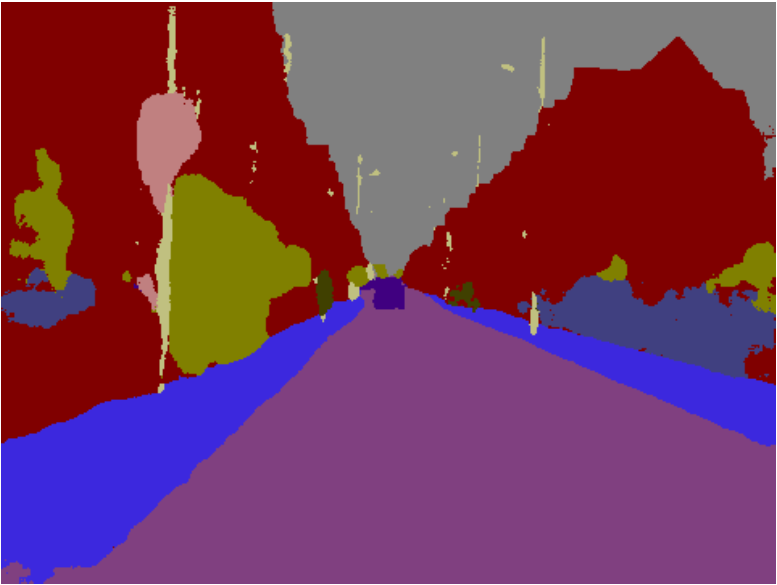
\includegraphics[width=.4\textwidth]{fig_3.png}}
\caption{Current Output [1].}
\end{figure}

\begin{figure}[h!]
\centering
\hyperlink{1}{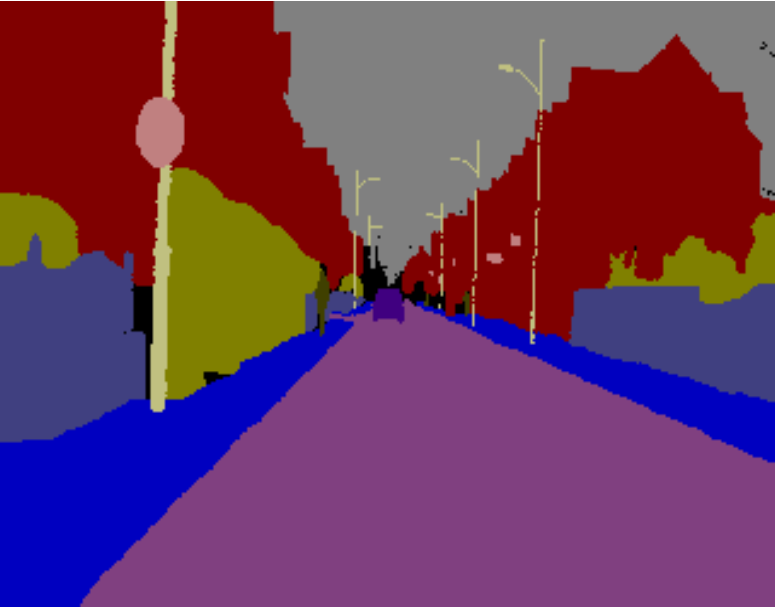
\includegraphics[width=.4\textwidth]{fig_4.png}}
\caption{Expected Output[1].}
\end{figure}

\clearpage

\section{References}
\setlength{\parindent}{4em}
\setlength{\parskip}{1em}
\begin{enumerate}

\item \hypertarget{1}{V. Badrinarayanan, A. Kendall, R. Cipolla, Senior Member, IEEE,\textit{ “SegNet: A Deep Convolutional Encoder-Decoder Architecture for Image Segmentation “}[2017 TPAMI] https://arxiv.org/abs/1511.00561. IEEE Transactions on Pattern Analysis and Machine Intelligence ( Volume: 39 , Issue: 12 , Dec. 1 2017 )}
\item \hypertarget{2}{V. Badrinarayanan, A. Kendall, R. Cipolla, Senior Member, IEEE, \textit{“SegNet: A Deep Convolutional Encoder-Decoder Architecture for Robust Semantic Pixel-Wise Labelling”}, https://arxiv.org/abs/1505.07293. Submitted on 27 May 2015}
\item \hypertarget{3}{C. Szegedy, W. Liu, Y. Jia, P. Sermanet, S. Reed, D. Anguelov, D. Erhan, V. Vanhoucke, and A. Rabinovich, \textit{“Going deeper with convolutions,”} in CVPR, pp. 1–9, 2015.}
\item \hypertarget{4}{K. Simonyan and A. Zisserman, \textit{“Very deep convolutional networks for large-scale image recognition,”} CoRR, vol. abs/1409.1556, 2014.}
\item \hypertarget{5}{C. Farabet, C. Couprie, L. Najman, and Y. LeCun, \textit{“Learning hierarchical features for scene labeling,”} IEEE PAMI, vol. 35, no. 8, pp. 1915–1929, 2013.}
\item \hypertarget{6}{C. Liang-Chieh, G. Papandreou, I. Kokkinos, K. Murphy, and A. Yuille, \textit{“Semantic image segmentation with deep convolutional nets and fully connected crfs,”} in ICLR, 2015.}
\item \hypertarget{7}{K. Simonyan and A. Zisserman, \textit{“Very deep convolutional networks for large-scale image recognition,”} arXiv preprint arXiv:1409.1556, 2014.}
\item \hypertarget{8}{O. Russakovsky, J. Deng, H. Su, J. Krause, S. Satheesh, S. Ma, Z. Huang, A. Karpathy, A. Khosla, M. Bernstein, A. C. Berg, and L. Fei-Fei, \textit{“ImageNet Large Scale Visual Recognition Challenge,”} International Journal of Computer Vision (IJCV), pp. 1–42, April 2015.}
\item \hypertarget{9}{S. Ioffe and C. Szegedy, \textit{“Batch normalization: Accelerating deepnetwork training by reducing internal covariate shift,”} CoRR, vol. abs/1502.03167, 2015.}

\end{enumerate}


\end{document}